\documentclass[12pt, oneside, a4paper]{book}

\usepackage{sectsty}

\chapternumberfont{\Large} 
\chaptertitlefont{\huge}

% Set input encoding
\usepackage[utf8]{inputenc}
% For coloured text and backgrounds
\usepackage[table, xcdraw]{xcolor}
% To create compact lists
\usepackage{paralist}
% To get current date and time
\usepackage{datetime}
% To include graphics
\usepackage{graphicx}
% To allow for easier positioning of graphics
\usepackage[export]{adjustbox}
% Nested Lists
\usepackage{outlines}
\usepackage{hyperref}
\usepackage{geometry}
\geometry{
    a4paper,
    left={35mm},
    top={25mm},
    right={25mm},
    marginparwidth={0cm},
    headheight={15pt}
}
% Place figures where they are supposed to be placed
\usepackage{float}

% To add caption and labels to the tables
\usepackage{booktabs}
\usepackage{caption2}

\renewcommand{\listfigurename}{\section{Illustration Directory}}
\renewcommand{\listtablename}{\section{Table Directory}}

% To allow multiple columns in itemize
\usepackage{multicol}
\setlength{\columnsep}{5pt}

% Change the Space before Chapters
\usepackage{etoolbox}
\makeatletter
\patchcmd{\@makechapterhead}{\vspace*{50\p@}}{}{}{}%
\patchcmd{\@makeschapterhead}{\vspace*{50\p@}}{}{}{}%
\makeatother

%Command to add Signatures
\newcommand*{\SignatureAndDate}[1]{%
    \par\noindent\makebox[2.5in]{\hrulefill} \hfill\makebox[2.0in]{\hrulefill}%
    \par\noindent\makebox[2.5in][l]{#1}      \hfill\makebox[2.0in][l]{Date}%
}%

\hypersetup{
    pdfauthor = {Gianluca Nenz, Ronny Mueller, Thomas Kleb}
    pdftitle = {Studienarbeit HS22}
}

% Header and Footer Styling
\usepackage{fancyhdr}
\pagestyle{fancy}
\fancyhf{}
\fancyhead[L]{\leftmark}
\fancyhead[R]{G.Nenz, R. Mueller, T.Kleb}
\fancyfoot[C]{\thepage}

\usepackage[
    style=ieee,
    backend=biber
]{biblatex}
\addbibresource{references.bib}


\begin{document}

% Changes numbering to lowercase roman.
\frontmatter


% Title Page
\begin{titlepage}

    \begin{center}

        
\includegraphics[height=0.15\textwidth, right]{resources/ost-logo.png}

        \vspace{2.5 cm}

        \hrule
        \vspace{0.8cm}
        {\Huge Reverse Engineering Labs}
        \vspace{0.8cm}
        \hrule
        \vspace{1.5cm}

        {\LARGE Studienarbeit}

         
        \vspace{1 cm}

        Department for Computer Science \\
        OST - Ostschweizer Fachhochschule \\
        Campus Rapperswil-Jona \\

        \vspace{1 cm}

        Semester: Autumn 2022

        \vspace{3 cm}
        
        \begin{table}[h!]
            \centering
            \begin{tabular}{@{}ll}
                \textbf{Autors:}    & Gianluca Nenz \\
                                          & Ronny Mueller \\
                                          & Thomas Kleb \\
                                          &                    \\
                \textbf{Project Advisor:} & Ivan Buetler \\
                \textbf{Release:} & E-Prints \\
                \textbf{Version:} & \today
            \end{tabular}
        \end{table}
        

        \vfill

        % 
\includegraphics[height=2cm]{resources/ost-logo.png}\\

        \vspace{1cm}
        Department for Computer Science\\
        OST Eastern Switzerland University of Applied Sciences

    \end{center}

\end{titlepage}

\chapter{Abstract}
\begin{table}[H]
    \begin{tabular}{lp{0.78\linewidth}}
    \textbf{Background} & As it stands today there is no module or learning unit at the OST to teach the concept of software reverse engineering. \\
    \\
    \textbf{Purpose}    & Because reverse engineering is an important topic in the cybersecurity space, the goal of this SA is to create challenges in the topic of reverse engineering. These challenges will or can be used by lecturers of the OST in Rapperswil-Jona to teach the basics to the students. \\
    \\
    \textbf{Methods}    & To achieve this goal we created challenges in ascending difficulty. At first the students will get information about the software they will use and the overall strategies of reverse engineering. After that they learn about some more advanced concepts. The focus here is creating the challenges in a manner, which should teach the basics in a easy to understand fashion. These challenges will be hosted on the Hacking-Lab platform. To ensure the quality of our challenges we did organise testing participants, who are cybersecurity students in their fifth semester as well. These tests should be the indicator if the goal was reached. \\
    \\
    \textbf{Results}    & The primary goal was to create a total of up to 10 challenges in this SA. This goal was achieved with a total of 11 created challenges. The testing was also successfully carried out and the feedback overall positive. If there was some common feedback, we adjusted the corresponding challenge based on it. The chapter [section \ref{sec:testing}] covers this in detail. \\
    \\
    \textbf{Conclusions} & This project was overall very successful, but there has also to be said that the topic of reverse engineering is huge and only a very small portion of it was covered in these challenges. There are many more techniques and tools which have not been covered yet and this could be a future work. 
    \end{tabular}
    \end{table}


%Sets the Depth of the ToC (set to 2 to allow subsections)
\setcounter{tocdepth}{1}
\tableofcontents


\mainmatter


\chapter{Project Idea}
\section{Task}
\label{sec:task}
The goal of this project is to create a reverse engineering lab. The students who take part in the labs should learn reversing step by step and get comfortable with tools like IDA Freeware, Radare2, Hopper or Ghidra. The labs should primarily be completed on either a Windows or a Linux system. \\
After a first analysis, the requirements for the reverse engineering labs and the exercises should be formulated. Afterwards the students should create 8 - 10 engineering labs. It is important that theres a common thread through all the labs. The participating students should start with easier examples and slowly solve more complex tasks. ASLR and DEP should be a part of the labs.

\section{Problem Domain}
\label{sec:problem-domain}
To have an easy overview of the lab structure, a problem domain was created (see figure \ref{fig:mindmap}) at the beginning of the project. This ensured the projects goal is reached at the end. In addition to that, this mindmap is displayed in each of the labs to show the participating student which part of reverse engineering is taught.
\begin{figure}[H]
    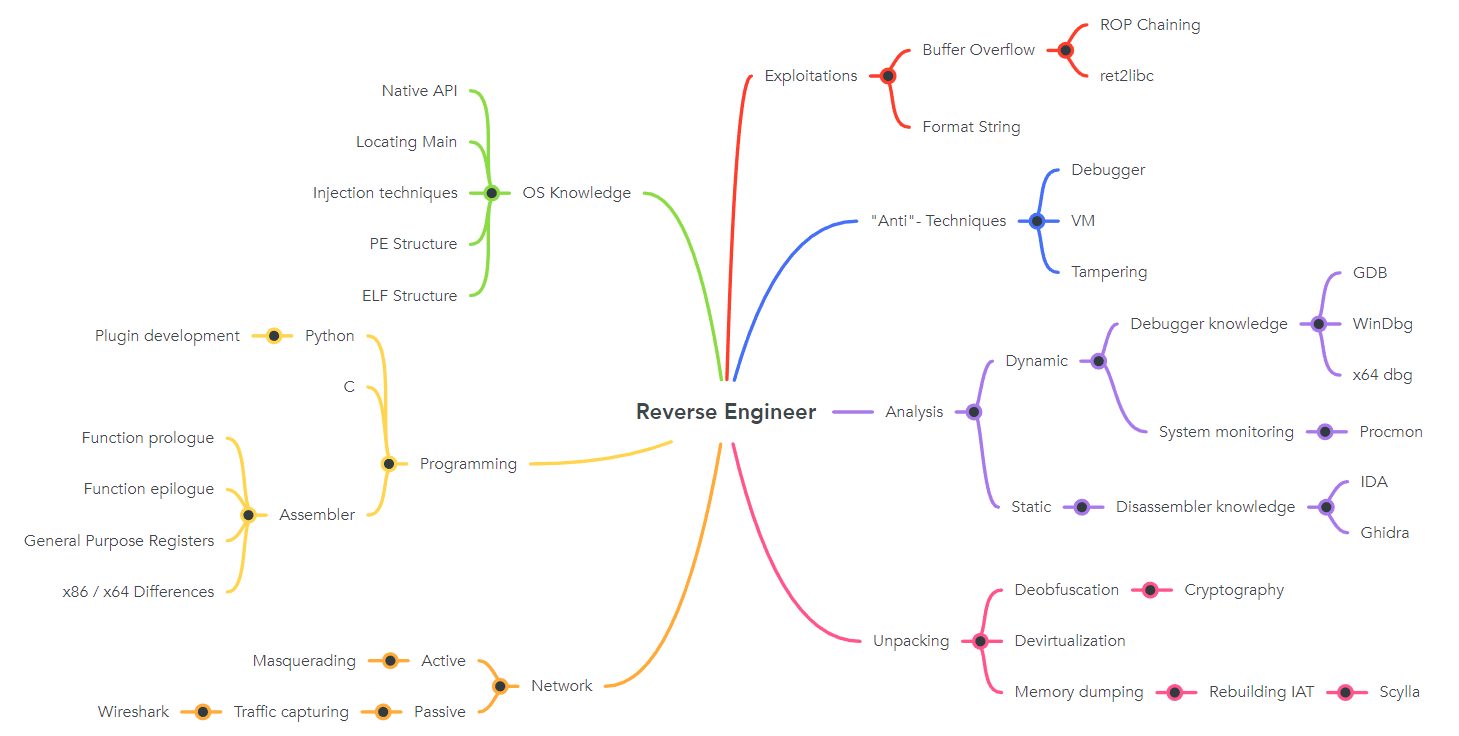
\includegraphics[width=\linewidth, center]{resources/RE_Domain_Light.png}
    \caption{Mindmap of the knowledge a reverse engineer needs.}
    \label{fig:mindmap}
\end{figure}

\section{Learning Concepts}
Before each lab is created a proof of concept (POC) has to be defined. These concepts contain the information about which part of the problem domain in figure \ref{fig:mindmap} is taught, how the lab is structured and what the teacher has to explain beforehand. The lab names and content were defined in a way that the student solving them has a clear thread to follow and goes from easier to harder exercises. \\
To assure the labs could be completed as planned it is assumed that the students have a basic knowledge in assembly language (ASM), Python and C. Since ASM is the most important language to understand the fundamental structure of a binary, a lab for refreshing this knowledge is planned.\\
The lab titles and content changed over the time of the project and the final scope of the labs differs from the one at the beginning. The final list is shown in table \ref{tab:labs}. 

\begin{center}
    \begin{table}[H]
        \centering
        \begin{tabular}{ |p{4.1cm}|p{10cm}| } 
            \hline
                Topic & 
                Description \\ [0.5ex] 
            \hline
            \hline
                Tutorial for the tools: GDB & Introduction into GDB and its tools \\
            \hline
                Tutorial for the tools: x64dbg & Introduction into x64dbg and how to navigate the GUI \\
            \hline
                Tutorial for the tools: IDA Freeware & Introduction into IDA Freeware and how to navigate the GUI \\
            \hline
                Refresher & 
                Give the students some little refreshing on the key topics (Assembly)  \\ 
            \hline
                Static Debugging & 
                Given a simple C file, students analyse it and try to find a key (Find Main function) \\ 
            \hline
                Dynamic Debugging & 
                Given a simple C file, students analyse it and try to find a key (go more into GDB / x64) \\ 
            \hline
                First RE attempts & 
                Given simple files compiled in different compilers to find a key \\ 
            \hline
                Remote Login  & 
                Inspecting binary locally and using RE to gain access to a remote docker-container \\
            \hline
                Pwntools & 
                Exploiting a vulnerability found through RE with pwntools \\
            \hline
                AES Encryption & 
                Not only finding out the password but writing a keygen for the program \\
            \hline
                Patching a Binary & 
                Introduce new native API funcs / techniques like stack strings \\
            \hline
        \end{tabular}
        \caption{Overview of all the Labs.}
        \label{tab:labs}
    \end{table}
\end{center}


\chapter{Management Summary}
\section{Overview}
\subsection{What is Reverse Engineering}
Reverse engineering is the process of analyzing a product or system in order to understand how it works, how it was made, or how it can be improved. It involves taking apart the product or system, examining its components, and understanding how they fit together and interact with each other. \\
In the context of software, reverse engineering is the process of analyzing a computer program in order to understand how it works and how it was implemented. This may involve disassembling the program, studying its code and documentation to recreate or modify it. Reverse engineering can be driven by various motivations: learning about new technologies, fixing flaws / security vulnerabilities or creating competing products. \\  
Most of the time, reverse engineering is a challenging and time-consuming process, as it requires a deep understanding of the underlying technologies and systems. It is often used by experts in fields such as computer science, engineering, and security. 

\subsection{Current Situation}
For a computer scientist, it is always useful to have knowledge in cybersecurity subjects. To accomplish the task of showing the students the world of cybersecurity, the Ostschweizer Fachhochschule (OST) implemented several modules like "Cyber Security", "Secure Software" and the newest one "Cyber Defense". In these modules, the professors explained the different aspects using Hacking-Lab as platform for the exercises. The plan is to extend the current state with reverse engineering labs and exercises. The goal of them is to bring the students closer to this subject and explain the fundamentals of reverse engineering.

\section{Approach}
To achieve these tasks, new exercises will be added to Hacking-Lab OST environment, which is, as mentioned above, a platform with which students are already accustomed to. These exercises will be added in the form of challenges for the student to go through and will be built with the idea of future additions in mind.

\section{Procedure}
At the start of the project, the scope was defined. The defined scope was the base on which the labs are created. This scope includes the difficulty increase between each lab, the know how to be taught to understand the procedure and which tools are used by the student to finish the tasks. In addition to these points, a platform on which the student is intended to work on is defined.
For the students to solve the given tasks, they needed a provided infrastructure to follow.

\section{Technologies}
The labs are created using either the Windows or Linux operating system, depending on the software needed. This allows the solving student to have the option to complete each lab on one of the two systems using a virtual machine if needed. 
All the labs are hosted on a Hacking-Lab tenant provided by the advisor, first on demo to test all the features and how to set them up, then on the OST tenant for official use. \\
Hacking-Lab is a website that offers a range of cybersecurity-related services, including training, simulations, and challenges. It is designed for professionals in the cybersecurity field, as well as students and enthusiasts who are interested in learning about and improving their skills in this area.
Because of this, the OST uses it to host different exercises to teach the fundamentals of cybersecurity to its interested students.

\section{Results}
\subsection{Goals Achieved}
The goals were defined by the advisor in section \ref{sec:task}. It was planned to have 8 - 10 labs finished until the end of week 12. This goal was reached thanks to a strict plan and coordination between the students.

\subsection{Goals Not Achieved}
Some goals were redefined during the iterative process of the project, but in the end, all of them were reached successfully. During the project, 11 concepts were defined and uploaded to Hacking-Lab.

\section{Future}
The labs created in this project are a base for future labs and should show participating students the initial steps of reverse engineering. The students plan to further add to the labs in the bachelor thesis, together with going into more advanced subjects and more complicated exercises. 


\chapter{Technical Report}
\section{Introduction}
\subsection{Problem}
The subject of cybersecurity is constantly growing in importance for the computer scientist in general. The demand for cybersecurity experts with broad knowledge regarding current problems and malware is ever growing \cite{cybercrime-mag}. The Ostschweizer Fachhochschule (OST) has recognized this demand and has added more and more lectures for the cybersecurity interested students \cite{ost-cybersec}. One important aspect is still missing in the curriculum: reverse engineering.

\subsection{Similar Work}
To this date there is no work done regarding this subject in past projects. In the past, students have created different labs for the OST but none for reverse engineering. The infrastructure which is used for this project is already existing and established in the OST lectures. Hacking-Lab as the platform is known by the targeted student group and teachers alike. 

\subsection{Technologies Used}
To create each of the labs and their documentation multiple different tools and languages were used (shown in table \ref{tab:languages} and \ref{tab:tools}). 
\begin{center}
    \begin{table}[H]
        \centering
        \begin{tabular}{ |p{4.1cm}|p{10cm}| } 
            \hline
            \multicolumn{2}{||c||}{\textbf{Languages}} \\
            \hline
            \hline
                Assembler & As the base structure of a binary it was taught in multiple Courses before this. In the labs ASM is used to understand the flow of a function and what it does when executed. \\
            \hline
                C & All of the binaries were written in C.   \\
            \hline
                Python & As an easy to understand language Python is used to write the exploits after analyzing the binaries. \\
            \hline
        \end{tabular}
        \caption{Overview of all the languages used to create the labs.}
        \label{tab:languages}
    \end{table}
\end{center}

\begin{center}
    \begin{table}[H]
        \centering
        \begin{tabular}{ |p{4.1cm}|p{10cm}| } 
            \hline
            \multicolumn{2}{||c||}{\textbf{Tools}} \\
            \hline
            \hline
                VSCode & Each of the students of the project used VSCode for programming and documenting. This allowed for easier settings and more control of the output. \\
            \hline
                IDA Freeware & Each of the labs were tested before uploading to Hacking Lab. All of the tests were done in IDA Freeware since this software is used to show the solutions.  \\
            \hline
                Ghidra & Each of the labs were tested before uploading to Hacking Lab. Ghidra was used to check the pseudo code. This ensured that students using Ghidra instead of IDA Freeware have a solvable problem aswell and can follow the steps given. \\
            \hline
                HL Demo Tenant & 
                To test all of the labs, the demo tenant of Hacking Lab was used. This allowed for free testing without interfering with the OST tenant.  \\ 
            \hline
                Docker & Docker container can be used on the Hacking Lab platform to have a server side component to the challenges. \\
            \hline
                OST Gitlab & 
                To have versioning of the code OSTs Gitlab was used.  \\ 
            \hline
                Clockify & 
                This software allowed for time management. \\ 
            \hline
        \end{tabular}
        \caption{Overview of all the frameworks and tools used to create the labs.}
        \label{tab:tools}
    \end{table}
\end{center}

\subsection{Goals}
The goal for this project has multiple facets:
\begin{itemize}
    \item The creation of different labs to show the students of the OST the aspects of reverse engineering
    \item The students should have the following learning objectives:
    \begin{itemize}
        \item Gain an understanding of what reverse engineering is and what it can be used for
        \item Know the basic handling of debuggers and disassemblers
        \item Understand a binary programs control flow using static debugging
        \item Understand a binary programs control flow using dynamic debugging
        \item Be able to locate and exploit simple security flaws in a binary program.
    \end{itemize}
\end{itemize}

\subsection{Product}
Since every student uses his own machine with his own configurations, Hacking-Lab as a platform with its LiveCD was chosen as the foundation. This allows a simple, operating system independent approach to all excercises thanks to its webinterface and docker hosting capabilities. 

\section{Requirements for the Labs}

\subsection{Overview}
This chapter lists the different requirements we have defined in order to successfully create and solve the reverse engineering labs.
\subsection{Requirements}
\textbf{Language} \\
The labs and their solutions will be written in english to guarantee each student can understand it. \\[0.5cm]
\textbf{Targeted Group of Students} \\
The product of this project is aimed at students in their third year (fifth semester) or higher because it is an in-depth look at a cybersecurity subject. Students taking this course should have visited the mandatory subject "Cyber Security" to have basic information and maybe even "Secure Software" for more advanced knowledge of some exploitations. A rule of thumb is the more security lectures a student has visited and finished, the better. \\[0.5cm]
\textbf{Time Requirements} \\
Each of the labs has a different time requirement for the students. One lab should be solvable in an hour or less.  \\[0.5cm]
\textbf{Grading} \\
Depending on the lab, a student has to hand-in a flag and/or a writeup. These will be checked by the teacher or an automated system. \\[0.5cm]

\newpage
\section{Lab Documentation}
% ------------------------------------------ INTRODUCTIONS ------------------------------------------ %
\subsection{Tools Introduction: GDB}
\subsubsection*{Problem Domain}
This lab covers the following aspects of the reverse engineering problem domain created by us:
\vspace{-2ex}
\begin{figure}[H]
    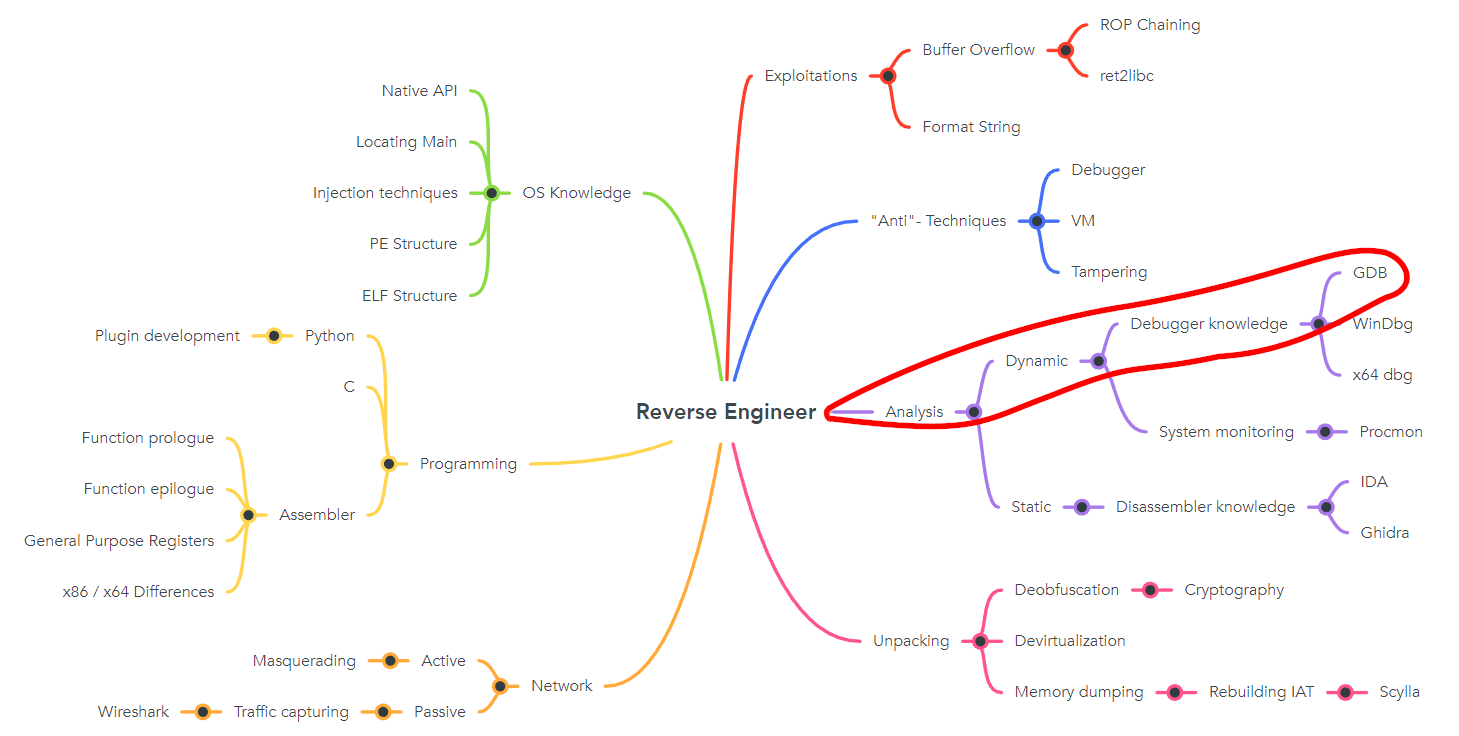
\includegraphics[width=\textwidth]{resources/GDBIntro-overview-light.png}
    \caption{GDB domain overview}
    \label{fig:gdb-overview}
\end{figure}
\subsubsection*{Content}
This introduction is used to explain the basic functionalities of the tool used in some of the labs. In this case GDB (GNU Debugger).
\subsubsection*{Choice of Topic}
The solutions and tips in the labs are given via screenshots or explanations. If a student wants to use a different tool he / she is free to do so. It is important that the tools used in the example solutions are known to the students. This makes it easier for them to understand each step and, if they are stuck at any point, follow the intructions on how to solve it. 
\subsubsection*{Objectives}
\begin{itemize}
    \item Learn about GDB and how to use the different commands available
\end{itemize}
\subsubsection*{Grading}
The labs are not graded since they are only used as a lookup. They have a flag to make sure the students have read the tools.
\pagebreak

\subsection{Tools Introduction: x64dbg}
\subsubsection*{Problem Domain}
This lab covers the following aspects of the reverse engineering problem domain created by us:
\vspace{-2ex}
\begin{figure}[H]
    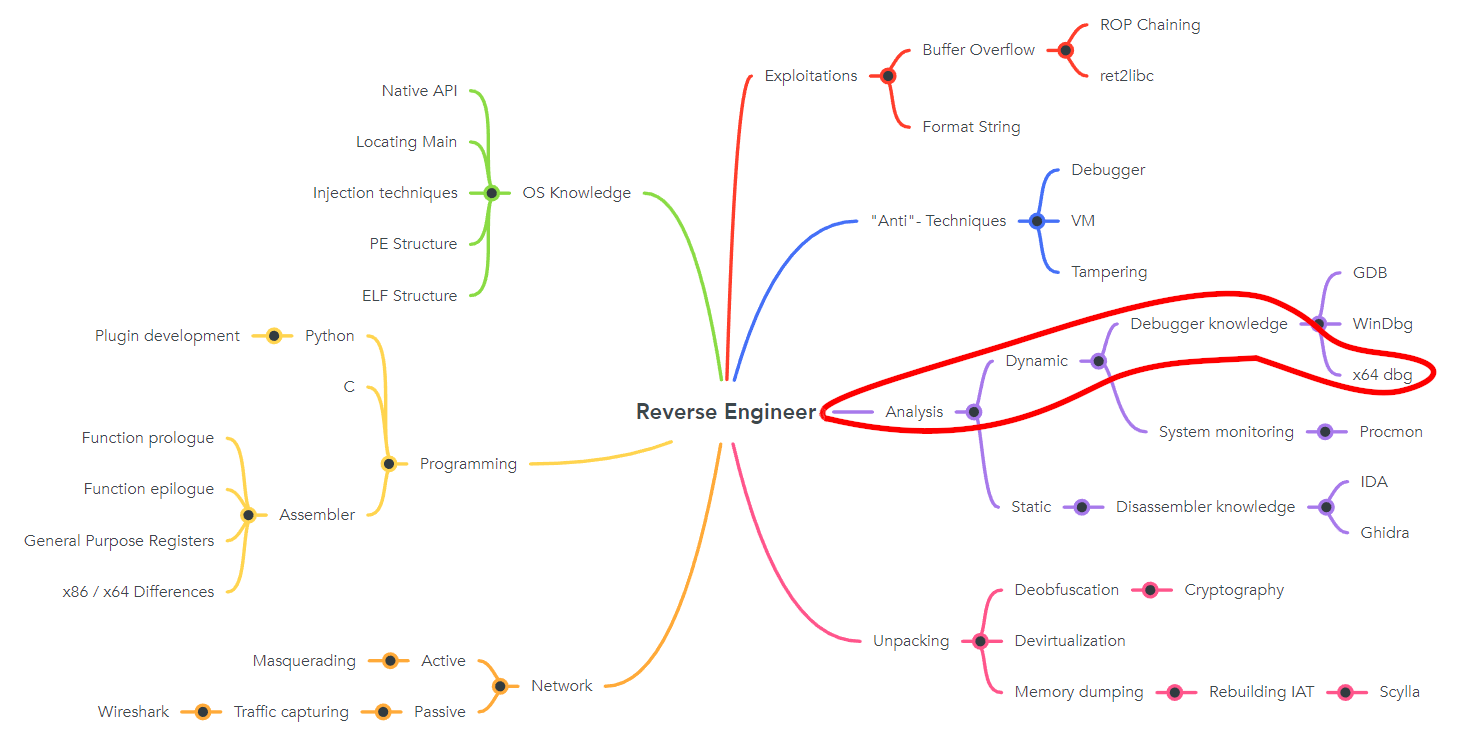
\includegraphics[width=\textwidth]{resources/x64Intro-overview-light.png}
    \caption{x64Intro domain overview}
    \label{fig:x64Intro-overview}
\end{figure}
\subsubsection*{Content}
Because most students have probably never touched a debugger on Windows before, this lab will help getting their feet wet with one of the most widely used ones by professionals.
This lab also acts as the basis for the upcoming labs where x64dbg will be used.
\subsubsection*{Choice of Topic}
Students working with Windows should also be given the opportunity to use a debugger. This lab will guide them through the GUI of the program and explain the basic functionality of what is coming up in future labs.
\subsubsection*{Objectives}
\begin{itemize}
    \item Install x64dbg and get a brief overview
    \item Get to know the functionality of x64dbg and be ready to use it on a binary
\end{itemize}
\subsubsection*{Grading}
The introduction labs are not graded since they are only used as a lookup. They have a flag to make sure the students have read the tools.
\pagebreak

\subsection{Tools Introduction: IDA Freeware}
\subsubsection*{Problem Domain}
This lab covers the following aspects of the reverse engineering problem domain created by us:
\vspace{-2ex}
\begin{figure}[H]
    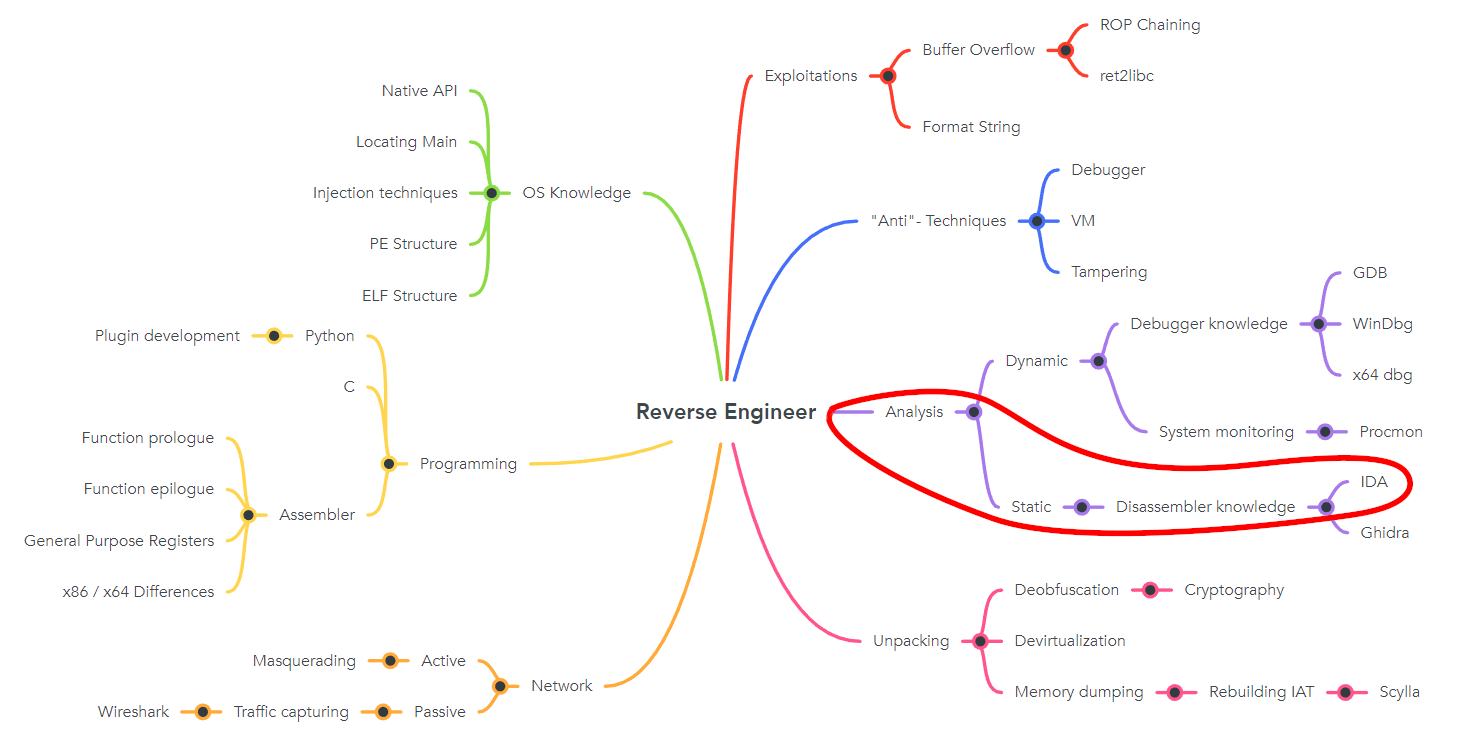
\includegraphics[width=\textwidth]{resources/IDAIntro-overview-light.png}
    \caption{IDAIntro domain overview}
    \label{fig:IDAIntro-overview}
\end{figure}
\subsubsection*{Content}
This introduction explains all the relevant functionalities of IDA and how to install it.
\subsubsection*{Choice of Topic}
Some of the Reverse Engineers most powerful tools are disassemblers. We purposely chose IDA Freeware over Ghidra for the beginning. This prevents the students from just generating pseudo code instead of actually reading and understanding the assembly instructions in later labs. Because of this, the solutions of future labs are presented using IDA Freeware.
\subsubsection*{Objectives}
\begin{itemize}
    \item Install IDA Freeware and get a brief overview
    \item Learn to orient yourself in IDA and get ready to use it on a binary.
\end{itemize}
\subsubsection*{Grading}
The introduction labs are not graded since they are only used as a lookup. They have a flag to make sure the students have read the tools.
\pagebreak
% ------------------------------------------ LABS ------------------------------------------ %

\subsection{Lab 1: Asm-Refresher}
\subsubsection*{Problem Domain}
This lab covers the following aspects of the reverse engineering problem domain created by us:
\vspace{-2ex}
\begin{figure}[H]
    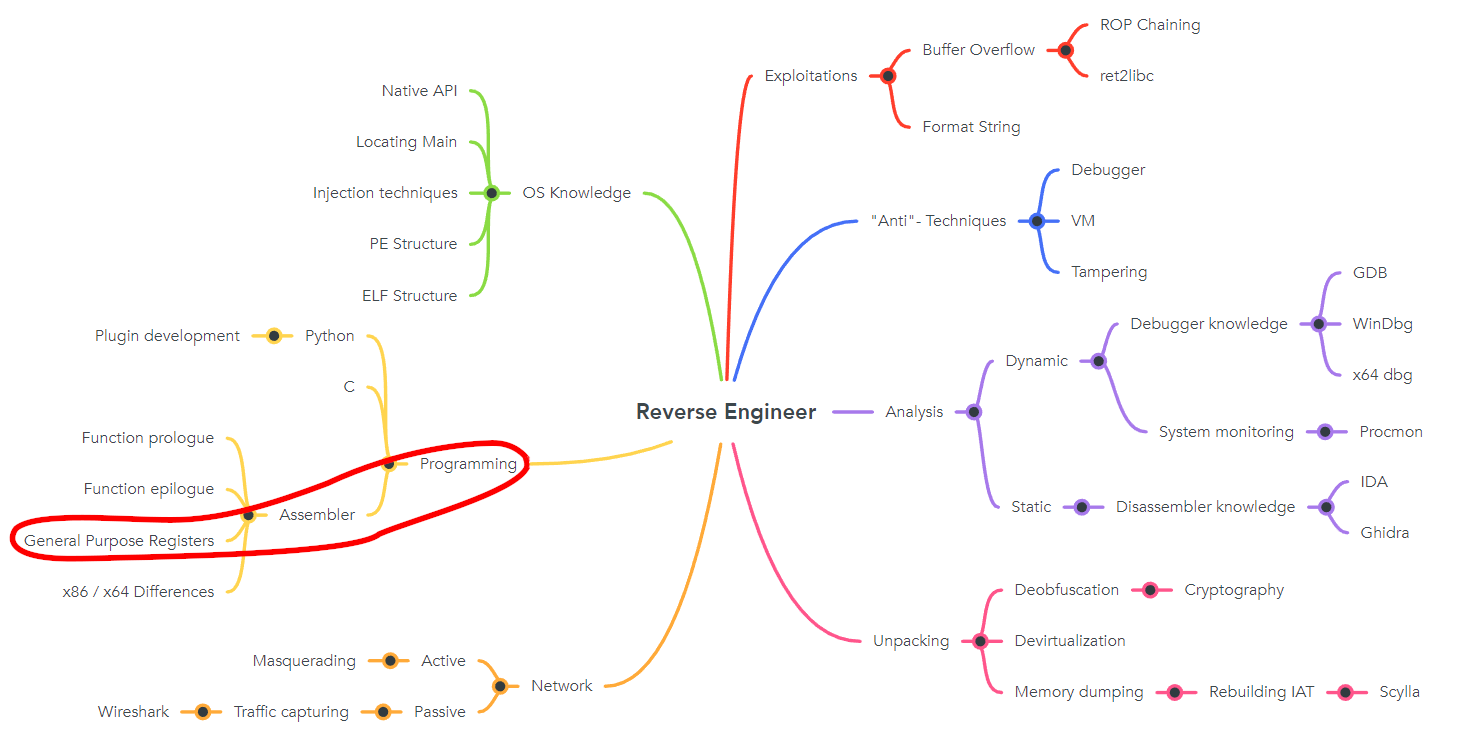
\includegraphics[width=\textwidth]{resources/ASM-overview-light.png}
    \caption{ASM refresher domain overview}
    \label{fig:refresher-overview}
\end{figure}
\subsubsection*{Content}
This lab is designed to be a refresher for those who have not done anything assembly related in a while. It covers the basic assembly instructions, explains the General-Purpose Registers and rounds up with a guide on how to write a "Hello World" program.  
\subsubsection*{Choice of Topic}
A reverse engineer has to understand the basic concepts of assembly. Not only when reading through dissasembled code but also later on when automatic pseudo code generation fails.
\subsubsection*{Objectives}
\begin{itemize}
    \item Refresh knowledge about the general-purpose registers.
    \item Basic understanding of assembly instructions
\end{itemize}
\subsubsection*{Grading}
This lab will not be graded since it is meant to help the students in later labs if they struggle with assembly.
\pagebreak

\subsection{Lab 2: Static Debugging}
\subsubsection*{Problem Domain}
This lab covers the following aspects of the reverse engineering problem domain created by us:
\vspace{-2ex}
\begin{figure}[H]
    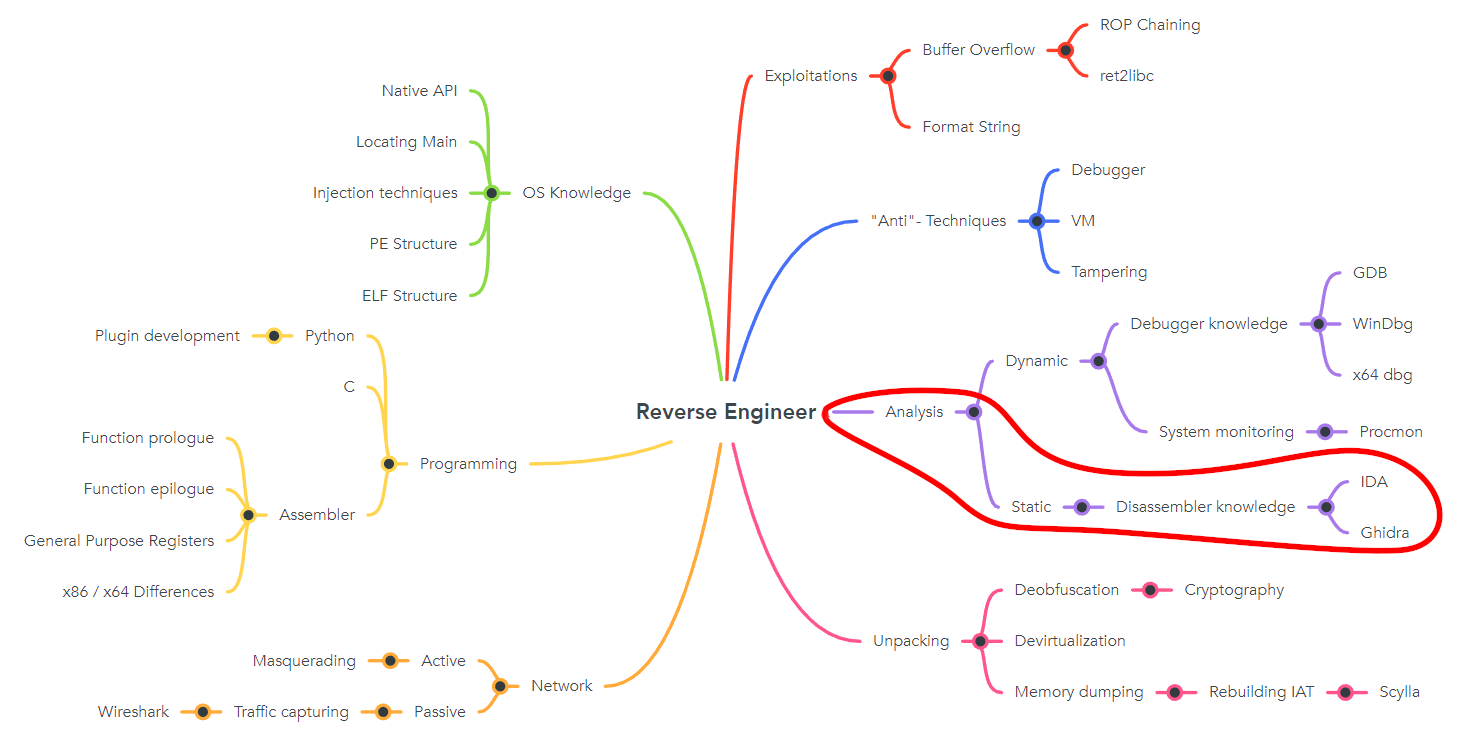
\includegraphics[width=\textwidth]{resources/static-overview-light.png}
    \caption{Static debugging domain overview}
    \label{fig:static-overview}
\end{figure}
\subsubsection*{Content}
In this lab the student will learn how to use IDA Freeware to statically reverse a given binary. The goal is to find the main function in a binary with and one without symbols. \\
This will show the student that seemingly simple things such as finding the main function can be a real problem if you have insufficient knowledge of the inner workings of a binary and the automatic detection of IDA fails.
\subsubsection*{Choice of Topic}
Program execution starts from the main() function which is why it is an important skill of a reverse engineer to find it and start understanding the rest of the binary from there on.
\subsubsection*{Objectives}
\begin{itemize}
    \item Find the main function in a normal binary
    \item Find the main function in a binary with symbols stripped
\end{itemize}
\subsubsection*{Grading}
The student has to inspect the main functions and find a flag in both of them. The final hand-in will be the combined flag.
\pagebreak

\subsection{Lab 3: Dynamic Debugging}
\subsubsection*{Problem Domain}
This lab covers the following aspects of the reverse engineering problem domain created by us:
\vspace{-2ex}
\begin{figure}[H]
    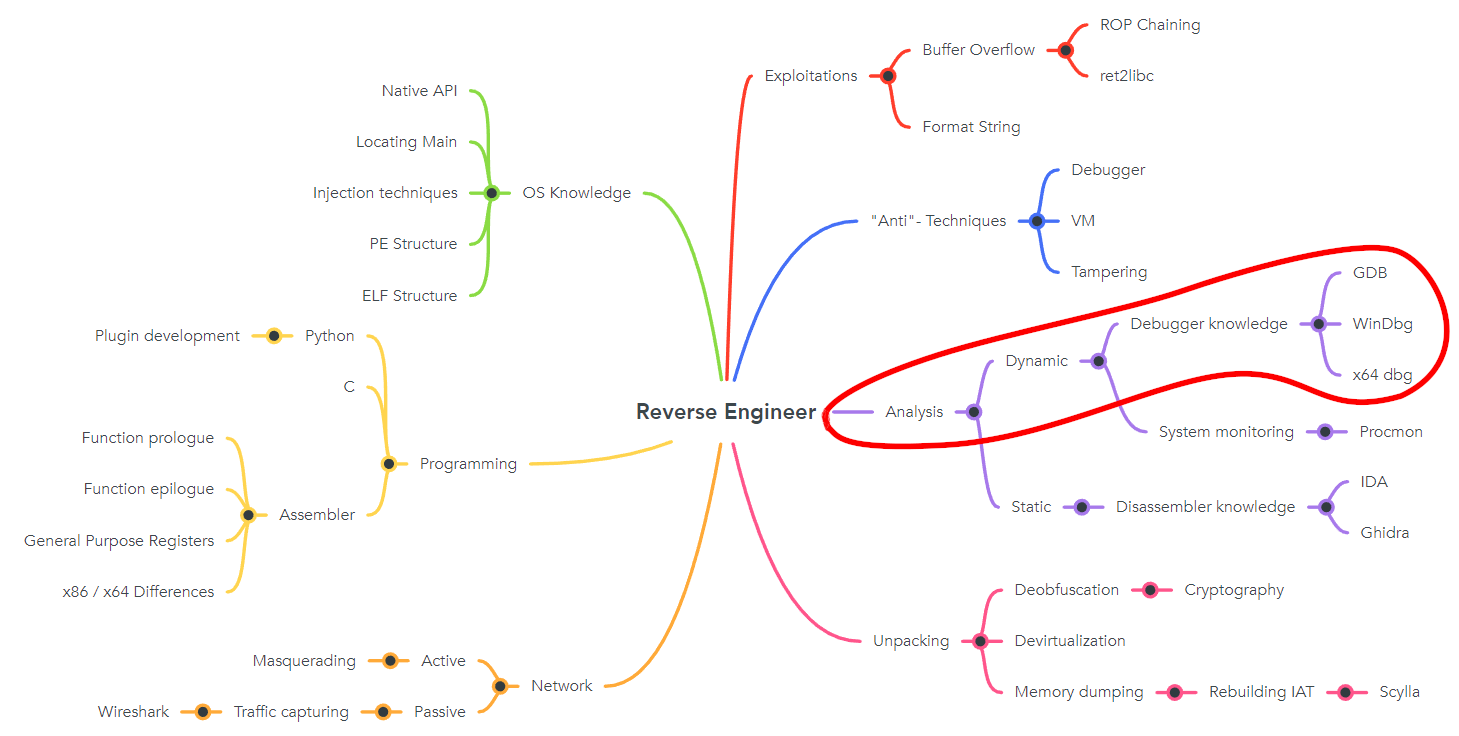
\includegraphics[width=\textwidth]{resources/dynamic-overview-light.png}
    \caption{Dynamic debugging domain overview}
    \label{fig:dynamic-overview}
\end{figure}
\subsubsection*{Content}
In this lab the student will learn how to use GDB and x64dbg to dynamically reverse a given binary. In a first step the lab explains how to dynamically debug the binary given in lab 2 and then, in a second step, the student will be presented with a new binary containing a flag. \\
The goal of this lab is to show the student how this skill is used and then have him do it on his own to solidify the steps he has completed before.
\subsubsection*{Choice of Topic}
Next to static debugging, dynamic debugging is used in a wide range of reverse engineering. Because of this it is important to have a student go through the steps and explain how it is done. 
\subsubsection*{Objectives}
\begin{itemize}
    \item Use GDB or x64dbg to find the flag of the binary
    \item Find the flag of a new binary using dynamic debugging
\end{itemize}
\subsubsection*{Grading}
The student has to use the newly aquired skills to find the flag in a new binary using dynamic debugging skills.
\pagebreak

\subsection{Lab 4: First Reversing Attempts}
\subsubsection*{Problem Domain}
This lab covers the following aspects of the reverse engineering problem domain created by us:
\vspace{-2ex}
\begin{figure}[H]
    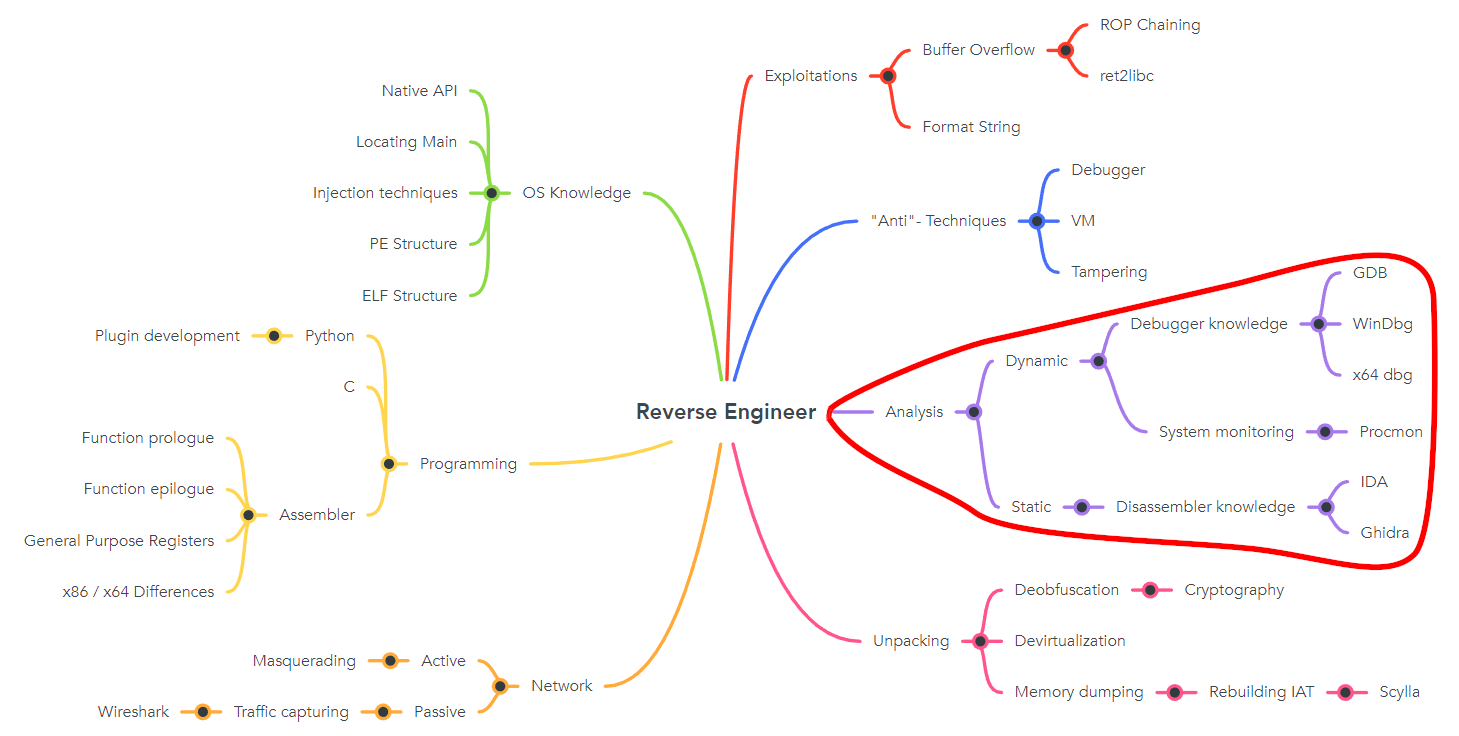
\includegraphics[width=\textwidth]{resources/reattempts-overview-light.png}
    \caption{RE attempts domain overview}
    \label{fig:reattempts-overview}
\end{figure}
\subsubsection*{Content}
In this lab the student will deepen his knowledge of reversing binaries to find out how they work. This challenge contains two binaries having different requirements that have to be met in order for the student to receive the flags.
\subsubsection*{Choice of Topic}
It is important to give the students simple examples where they can play around and learn by doing without providing a step by step guide.
\subsubsection*{Objectives}
\begin{itemize}
    \item Use static or dynamic debugging to find the requirements of the programs
    \item Find out how program arguments are handled in assembly
\end{itemize}
\subsubsection*{Grading}
The student has to solve both binaries to get a flag.
\pagebreak

\subsection{Lab 5: Remote Login}
\subsubsection*{Problem Domain}
This lab covers the following aspects of the reverse engineering problem domain created by us:
\vspace{-2ex}
\begin{figure}[H]
    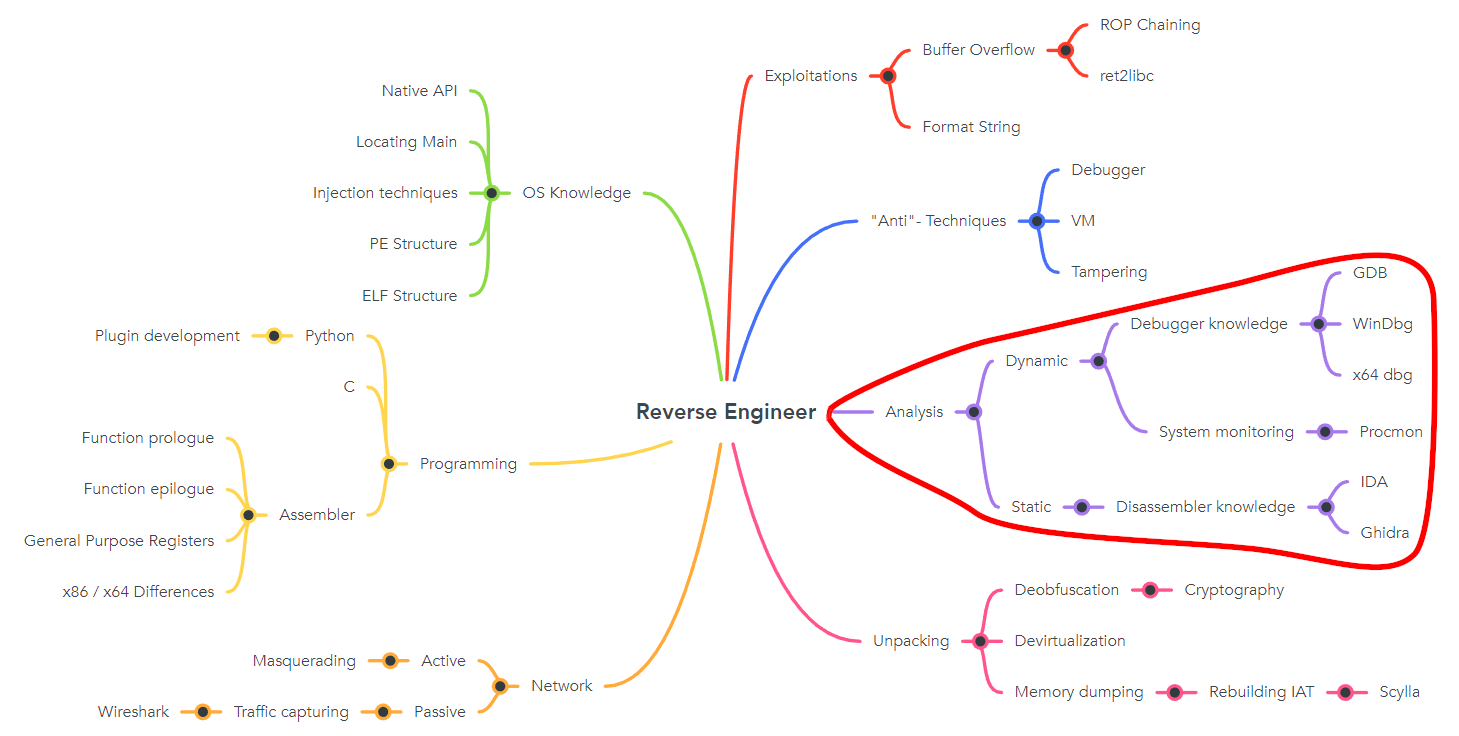
\includegraphics[width=\textwidth]{resources/remotelogin-overview-light.png}
    \caption{Remote login domain overview}
    \label{fig:remotelogin-overview}
\end{figure}
\subsubsection*{Content}
This lab dives deeper into the reverse engineering rabbit hole and introduces a new concept. The student first starts a docker container off a provided resource.
This docker container exposes a webserver and a port where an application runs. The application running on the server can be downloaded from the servers website by the student. \\
The student then has to combine dynamic and static reverse engineering to figure out the password in order to log into the server and expose the flag.
\subsubsection*{Choice of Topic}
Giving the students an idea that reverse engineering can be used to gather information that you can later exploit on a target system.
\subsubsection*{Objectives}
\begin{itemize}
    \item Learn to use the tools you got introduced to
    \item Apply basics of dynamic and static debugging and find a way to exploit remote target 
\end{itemize}
\subsubsection*{Grading}
The student has to find out the flag and submit a small writeup to answer the security questions provided.
\pagebreak

\subsection{Lab 6: Pwntools - Introduction}
\subsubsection*{Problem Domain}
This lab covers the following aspects of the reverse engineering problem domain created by us:
\vspace{-2ex}
\begin{figure}[H]
    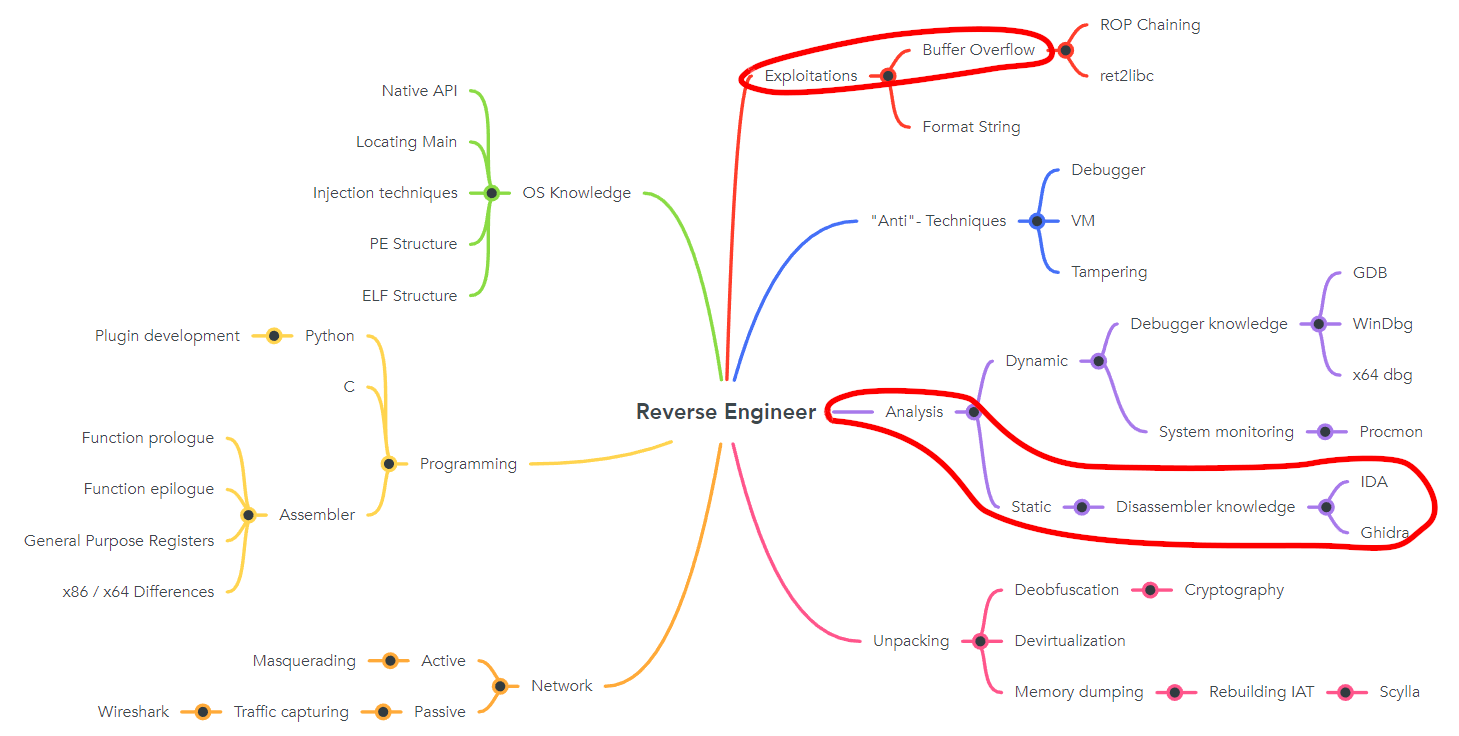
\includegraphics[width=\textwidth]{resources/pwntools-overview-light.png}
    \caption{Pwntools domain overview}
    \label{fig:pwntools-overview}
\end{figure}
\subsubsection*{Content}
In this lab the student has a first introduction into the pwntool module of python. The student first has to start a docker conatiner from the provided resource. This docker exposes both a webserver and a port where the application is running on. The student then downloads the compiled application to analyze it and search for a weakness to exploit. This weakness can then be exploited through the use of pwntools. Since this is a first introduction, the whole process of creating the script is guided as a walkthrough.
\subsubsection*{Choice of Topic}
Pwntools is an important module to learn for exploiting. Reverse engineering in general is widely used to find vulnerabilities to exploit, which means it is important for a student to not only know how to find the weakness but also how to exploit it.
\subsubsection*{Objectives}
\begin{itemize}
    \item Use acquired skills to find vulnerability in binary
    \item Create a pwntools script to exploit that vulnerabilty
\end{itemize}
\subsubsection*{Grading}
The grading is done by sending in the printed out flag when the script is run on the exposed port and a writeup answering the provided security questions.
\pagebreak

\subsection{Lab 7: Crypto Lab - AES ECB}
\subsubsection*{Problem Domain}
This lab covers the following aspects of the reverse engineering problem domain created by us:
\vspace{-2ex}
\begin{figure}[H]
    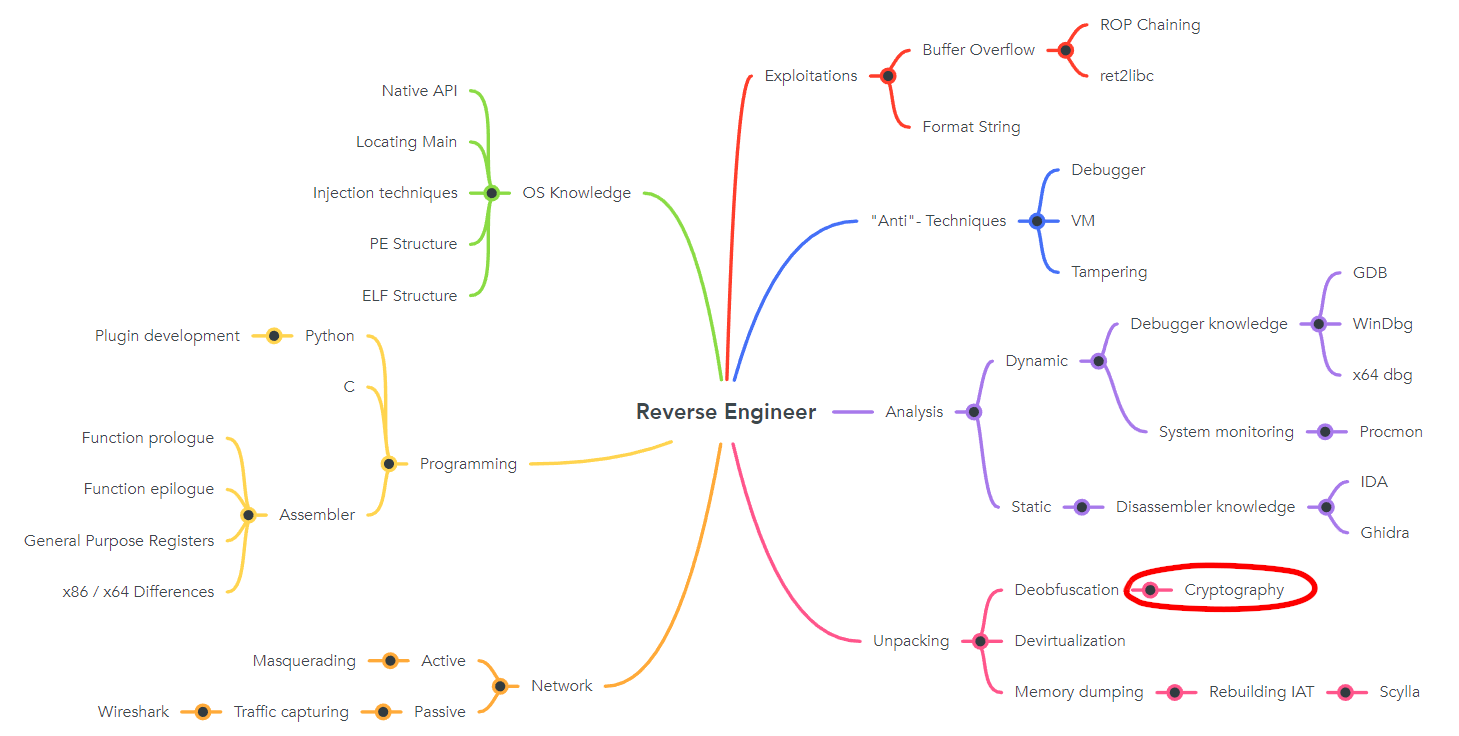
\includegraphics[width=\textwidth]{resources/aes-overview-light.png}
    \caption{AES domain overview}
    \label{fig:aes-overview}
\end{figure}
\subsubsection*{Content}
The student is presented a docker container which runs a webserver and exposes a port on which the script for the student to crack is running. The student first inspects and analyzes the script itself and then follows a walkthrough on how to write a simple script which exploits a common vulnerability in AES ECB mode. 
\subsubsection*{Choice of Topic}
Encryption is a widely used form of obfuscation. Because of this it is important as a cyber security student to be informed about certain weaknesses these ciphers have and how to exploit them if needed. 
\subsubsection*{Objectives}
\begin{itemize}
    \item Find out how the script works
    \item Find patterns to exploit
    \item Create a pwntools script to crack the encryption
\end{itemize}
\subsubsection*{Grading}
The grading is done by sending in the printed out flag when the script is run on the exposed port in combination with a writeup answering the provided security questions.
\pagebreak

\subsection{Lab 8: Patching Lab}
\subsubsection*{Problem Domain}
This lab covers the following aspects of the reverse engineering problem domain created by us:
\vspace{-2ex}
\begin{figure}[H]
    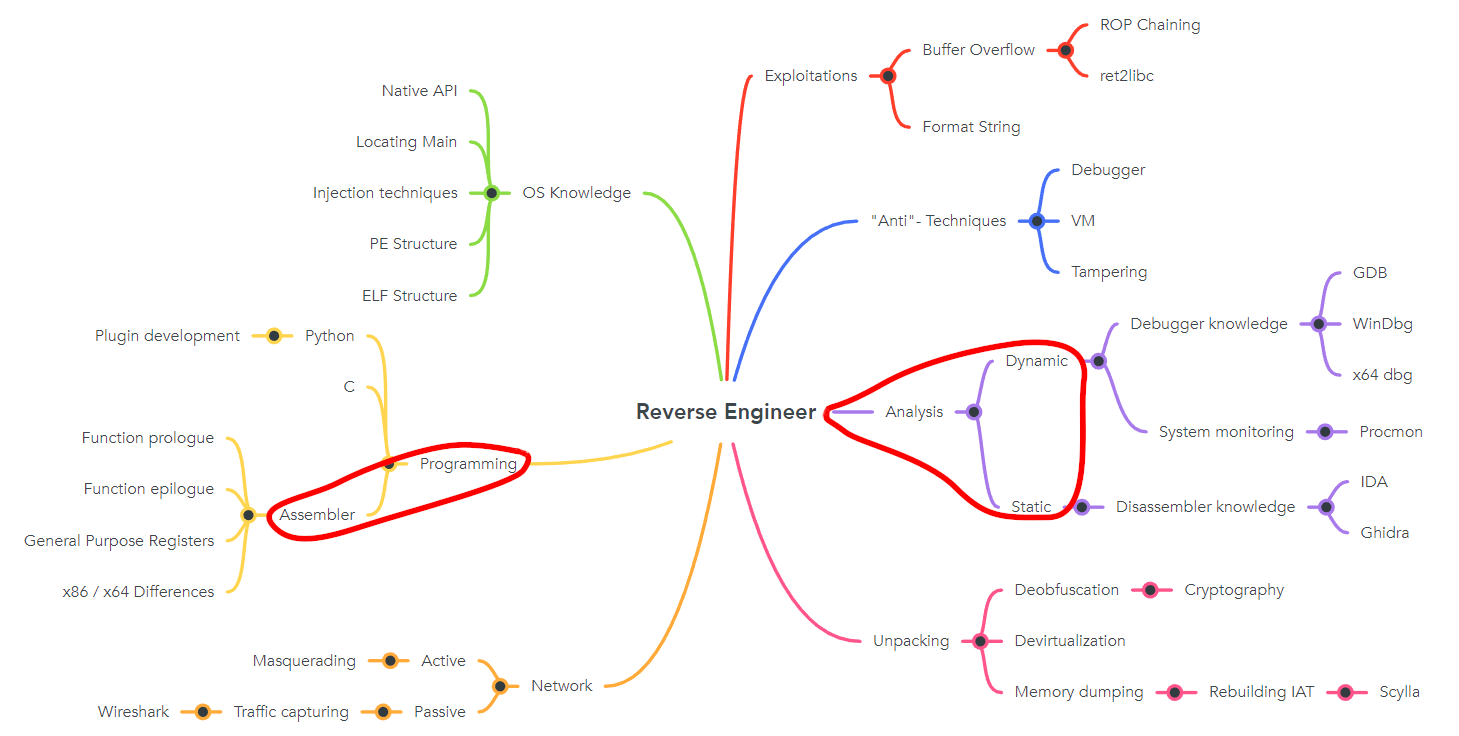
\includegraphics[width=\textwidth]{resources/patching-overview-light.png}
    \caption{Patching domain overview}
    \label{fig:patching-overview}
\end{figure}
\subsubsection*{Content}
The student is presented a binary which does not operate correctly. The student is tasked to find the location to patch and fix it. In order to check the patch generated by the user, the provided docker container starts up a webserver where the student can upload the patch file. The webserver then tries to apply the patch to a local copy of the binary and checks if the bug is fixed. If fixed, the webserver shows the flag to the student. If not fixed, the student has the possibility to reset the binary and try again.

\subsubsection*{Choice of Topic}
Reverse engineering also comes in handy when encountering bugs in software where the source code is unreachable. Therefore it is important to locate found bugs in an executable and know how to apply patches.
\subsubsection*{Objectives}
\begin{itemize}
    \item Find the mistake of the binary
    \item Change the ASM code and upload the patched file to the website
\end{itemize}
\subsubsection*{Grading}
The grading will be done via a writeup and a flag.
\pagebreak


% --------------------------------------%



\chapter{Project Documentation}
% --------------------------------------%
\section{Project Plan}
\subsection{Project Overview}
The goal of this project is to create and organize a lab, which shows and explains future students of the Ostschweizer Fachhochschule (OST) how reverse engineering is performed and which tactics are used to get information out of a program. To accomplish this task, the lab will have several exercises organized in the different domains. These exercises will be accessible through the Hacking-Lab hosted on the OST server. 

\subsubsection*{Hand-In}
The finished Report will be hended in according to the rules set by the "Studiengangsleitung Informatik" and the supervisor:
\begin{itemize}
    \item 2 PDF will be handed in. One for the supervisor and one for the archive.
    \item 1 printed version will be handed in to the supervisor for reading and grading.
\end{itemize}

\subsection{Management}
\subsubsection*{Time Management}
The project started on the first week of the semester (KW 38) and ends in week 51 giving us around 14 weeks to be done with the Hand-In. \\
Since the module has a total ECTS of 8 each of the students has to work around 240h during the semester which can be seen in table \ref{time_ects} together with the total planned time investment. This means, that per week each student should work around 17.1 hours.

\begin{table}
    \centering
    \begin{tabular}{||c c c c||} 
        \hline
        Name & ECTS & Time spent per Week [h] & Total Time spent [h]\\ [0.5ex] 
        \hline\hline
        Gianluca Nenz & 8 & 17.1 & 240 \\ 
        \hline
        Ronny Mueller & 8 & 17.1 & 240 \\
        \hline
        Thomas Kleb & 8 & 17.1 & 240 \\ 
        \hline
        \textbf{Total} & 32 & 52.3 & 720 \\[1ex] 
        \hline
    \end{tabular}
    \caption{Time Investments}
    \label{time_ects}
\end{table}

\subsubsection*{Planning}
In the past modules Software Engineering Practices 1 and 2 (SEP 1 + 2) we were introduced to different ways to plan and organize a project. The main tools we learned, RUP (Rational Unified Process) and Scrum, are mainly used in software development but can be adapted to other projects aswell. They both use different aspects of time management and organisation which is why we intend to apply them to our project.

\subsubsection*{\textit{RUP (Rational Unified Process)}}
\label{rup_section}
RUP is a process which allows a team to distribute a longterm plan over a given time and section it into multiple steps and parts. RUP has four main phases which have characteristics to be taken care of: \\

\vspace{0.2cm}

\noindent \textbf{Inception:} The goal in this phase is to propose the project, identifying the criterias to be assessed and a first estimation of risk and success. This part should take less than 5\% of the total time.\\
\textbf{Elaboration:} The elaboration phase is used to identify the requirements and the architecture. It should also be used to get rid or at least plan for the highest risks. After this phase the team has a plan of what to work on and how much work is to be done. This part should take about 25\% of the total time. \\
\textbf{Construction:} This step is where the team implements the functionality of the product and starts working on the development. A big part of it, is to get rid of risks which hinder the process. This is the biggest part, taking about 50\% of the total time.\\
\textbf{Transition:} This final step of RUP is ued to test the product and finalize the deployment. About 20\% of the time should be planned for it.\\

\pagebreak
\subsubsection*{\textit{Scrum}}
\label{scrum_section}
Scrum is a framework that helps teams work together. It is most frequently used by software development teams but its principles and lessons can be applied to all kinds of teamwork. It helps teams to find solutions for complex problems with the help of planning. It consists of different roles and parts to make it work:

\begin{multicols}{2}
    \begin{itemize}
        \item Scrum Team
        \begin{itemize}
            \item Developers
            \item Product Owner
            \item Scrum Master
        \end{itemize}
    \end{itemize}
    \begin{itemize}
        \item Scrum Events
        \begin{itemize}
            \item The Sprint
            \item Sprint Planning
            \item Daily Scrum
            \item Sprint Review
            \item Sprint Retrospective
        \end{itemize}
    \end{itemize}
    \columnbreak
    \begin{itemize}
        \item Scrum Artifacts
        \begin{itemize}
            \item Product Backlog
            \item Print Backlog
            \item Increment
        \end{itemize}
    \end{itemize}
    \begin{itemize}
        \item Scrum Values
        \begin{itemize}
            \item Commitment
            \item Focus
            \item Openness
            \item Respect
            \item Courage
        \end{itemize}
    \end{itemize}
\end{multicols}

\begin{figure}[h]
    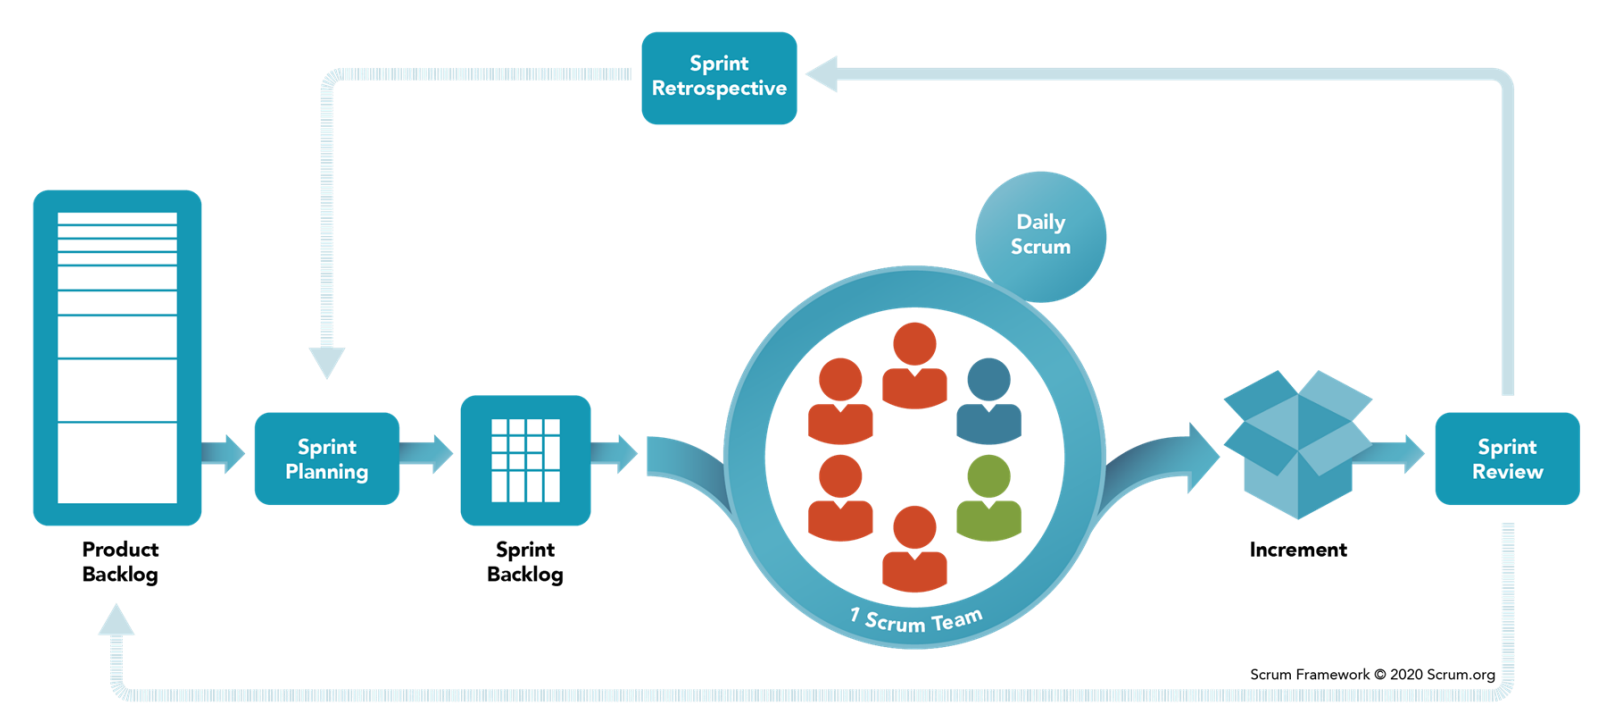
\includegraphics[width=\linewidth]{04_Project-Documentation/scrum.png}
    \caption{Scrum}
    \label{scrum_img}
\end{figure}
\subsection{Organisation}

\subsubsection*{Participants}
The "Studienarbeit"-Team consists of three students: Gianluca Nenz, Ronny Muel\-ler and Thomas Kleb. Work on the project and documentation will be evenly distributed between these three participants. Bigger decisions are made as a team in either the meetings with or without the advisor (the advisor will be notified on anyone made).

\subsubsection*{Advisor}
The teams advisor for the "Studienarbeit" is Ivan Buetler who is teaching cyber security modules at the OST.

\subsubsection*{Division of Labor}
The project has multiple facets that need to be taken care of. This is why the team has decided to distributed the work load between the three. This doesn't mean that the work is done by only the chosen student but rather that he is the one responsible that it works as planned.
\begin{table}[H]
    \begin{tabular}[t]{||p{4cm}||}
        \hline
        Gianluca Nenz \\
        \hline\hline
        Work 1 \\ 
        \hline
        Work 2 \\
        \hline
        Work 3 \\ 
        \hline
        Work 4\\[1ex] 
        \hline
    \end{tabular}
    \hfill
    \begin{tabular}[t]{||p{4cm}||}
        \hline
        Ronny Mueller \\
        \hline\hline
        Work 1 \\ 
        \hline
        Work 2 \\
        \hline
        Work 3 \\ 
        \hline
        Work 4\\[1ex] 
        \hline
    \end{tabular}
    \hfill
    \begin{tabular}[t]{||p{4cm}||}
        \hline
        Thomas Kleb \\
        \hline\hline
        Work 1 \\ 
        \hline
        Work 2 \\
        \hline
        Work 3 \\ 
        \hline
        Work 4\\[1ex] 
        \hline
    \end{tabular}
    \caption{Work Distribution per Student}
    \label{work_dis}
\end{table}

\subsection{Planning and Milestones}

\subsubsection*{Phases and Iterations}
The project is comprised of the four steps explained in \nameref{rup_section}. Each of those phases has multiple iterations which create the different sprints for the project. The meetings with the advisor will be on thursdays while the team meetings will be held tuesdays. Each iteration / sprint will be of a seven day length. \\

\noindent We started the "Studienarbeit" before we began with the regular school. In the week before we each made research and plans about the comming project. After having a talk with the advisor it was decided to first find out the level of knowledge each student has to make it easier for the advisor to plan.
\begin{table}[H]
    \centering
    \begin{tabular}{|p{0.1\linewidth}|p{0.15\linewidth}|p{0.15\linewidth}|p{0.46\linewidth}|}
        \hline
        \multicolumn{4}{||c||}{\textbf{Inception}} \\
        \hline \hline
        Iteration & Start & End & Description \\
        \hline \hline
        0 & 12.09.2022 & 18.09.2022 & Collection of Ideas and planning first meeting\\
        \hline
        1 & 19.09.2022 & 25.09.2022 & First meeting and handout of exercises to assess the knowledge of the students \\
        \hline
        2 & 26.09.2022 & 02.10.2022 & Working on the exercises and receiving solutions for harder ones \\
        \hline
    \end{tabular}
    \caption{RUP: Inception Phase Planning}
    \label{inception_table}
\end{table}

\noindent The elaboration phase is used to plan and assess the possible risks in this project. This consists of a documentation structure, the project plan and the risk management to make sure the construction phase has no major hickups.
\begin{table}[H]
    \centering
    \begin{tabular}{|p{0.1\linewidth}|p{0.15\linewidth}|p{0.15\linewidth}|p{0.46\linewidth}|}
        \hline
        \multicolumn{4}{||c||}{\textbf{Elaboration}} \\
        \hline \hline
        Iteration & Start & End & Description \\
        \hline \hline
        3 & 03.10.2022 & 09.10.2022 &  First big meeting with advisor; Creating project plan and risk analysis.\\
        \hline
        4 & 10.10.2022 & 16.10.2022 & ---- \\
        \hline
        5 & 17.10.2022 & 23.10.2022 & ---- \\
        \hline
    \end{tabular}
    \caption{RUP: Elaboration Phase Planning}
    \label{elaboration_table}
\end{table}

\noindent The construction phase is where the labs are primarily built. 
\begin{table}[H]
    \centering
    \begin{tabular}{|p{0.1\linewidth}|p{0.15\linewidth}|p{0.15\linewidth}|p{0.46\linewidth}|}
        \hline
        \multicolumn{4}{||c||}{\textbf{Construction}} \\
        \hline \hline
        Iteration & Start & End & Description \\
        \hline \hline
        6 & 24.10.2022 & 30.10.2022 & ----\\
        \hline
        7 & 31.10.2022 & 06.11.2022 & ---- \\
        \hline
        8 & 07.11.2022 & 13.11.2022 & ---- \\
        \hline
        9 & 14.11.2022 & 20.11.2022 & ---- \\
        \hline
        10 & 21.11.2022 & 27.11.2022 & ---- \\
        \hline
        11 & 28.11.2022 & 04.12.2022 & ---- \\
        \hline
    \end{tabular}
    \caption{RUP: Construction Phase Planning}
    \label{construction_table}
\end{table}

\noindent To make sure enough time is planned a buffer week was added to the transition phase. This phase is also mainly used to finish up the documentation and implement the different labs to Hacking Lab. The last week is used to clean up and hand in the documentation and abstract to both the OST and the advisor.
\begin{table}[H]
    \centering
    \begin{tabular}{|p{0.1\linewidth}|p{0.15\linewidth}|p{0.15\linewidth}|p{0.46\linewidth}|}
        \hline
        \multicolumn{4}{||c||}{\textbf{Transition}} \\
        \hline \hline
        Iteration & Start & End & Description \\
        \hline \hline
        12 & 05.12.2022 & 11.12.2022 & Buffer \\
        \hline
        13 & 12.12.2022 & 18.12.2022 & ---- \\
        \hline
        14 & 19.12.2022 & 23.12.2022 & ---- \\
        \hline
    \end{tabular}
    \caption{RUP: Transition Phase Planning}
    \label{transition_table}
\end{table}

\subsubsection*{Milestones}
To guarantee the success of the project milestones were defined with a deadline.

\begin{table}[H]
    \centering
    \begin{tabular}[]{|| p{5cm} | c | p{6.2cm} ||}
        \hline
        Milestones & Deadline & Description \\
        \hline \hline
        M1 - Solving RE Exercises & 05.10.2022 & The Team solves the given exercises to find the level of RE knowledge. \\
        \hline
        M2 - Defining Problem Domains and Learnconcepts& ---- & ---- \\
        \hline
        M3 - Lab Concepts & ---- & ---- \\
        \hline
        M4 - Refining Labs & ---- & ---- \\
        \hline
        M5 - Setup Labs& ---- & ---- \\
        \hline
        M6 - Hand-In& ---- & ---- \\
        \hline
    \end{tabular}
\end{table}

\subsubsection*{Time Tracking}
For time tracking the team has decided on using GitLabs integrated time tracking. 
\subsubsection*{Issue Tracking}

\subsubsection*{Meetings}
The team has meetings each tuesday to elaborate problems and check up on the progress. This meetings are also used to distributed the work load and the different parts of the sprint. \\
On Thursdays the team meets the advisor Ivan Buetler to inform him on the progress done and the problems that came up. These meetings have different time schedules to fit everyones calender. \\
Each meeting will be documented and uploaded to the GIT repository. After each meeting the participants should know what to do and how to contact each other if any problems arise.
\subsubsection*{CI/CD}

\subsubsection*{Testing}

\subsubsection*{Projectmanagment}
The whole project will use a GitLab repository. To make sure no confusion happens a multirepo principle is used where one repository is for the documentation and protocols only and other are for code, information gathered, etc. Each student works on a branch and before pushing to the main branch has another student look into the code / text written. 
% --------------------------------------%
\section{Risk Analysis}

\section{Project Monitoring}

\subsubsection*{Overview}

\subsubsection*{Milestones}

\subsubsection*{Time Tracking}

% --------------------------------------%
\section{Personal Rapports}

\subsubsection*{Gianluca Nenz}

\subsubsection*{Ronny Mueller}

\subsubsection*{Thomas Kleb}

\chapter{Meetings}
\section{06-10-22}
Lorem Ipsum


\backmatter

\chapter{Directory}

\phantomsection
\addcontentsline{toc}{section}{Glossary}
\section*{Glossary}

\phantomsection
\addcontentsline{toc}{section}{Bibliography}
% https://www.overleaf.com/learn/latex/Bibliography_management_in_LaTeX
\printbibliography


\chapter{Appendix}

\phantomsection
\addcontentsline{toc}{section}{Eigenständigkeitserklärung}
\section*{Eigenständigkeitserklärung}
Eigenständigkeitserklärung

\vspace{2 cm}

\noindent \textbf{Erklärung} \\
Wir erklären hiermit, \\

\begin{itemize}
    \item dass wir die vorliegende Arbeit selbst und ohne fremde Hilfe durchgeführt haben, ausser derjenigen, welche explizit in der Aufgabenstellung erwähnt ist oder mit de Betreuer schriftlich vereinbart wurde,
    \item dass wir sämtliche verwendeten Quellen erwähnt und gemäss gängigen wissen\-schaftlichen Zitierregeln korrekt angegeben haben.
    \item dass wir keine duch Copyright geschützten Materialien (z.B. Bilder) in dieser Arbeit in unerlaubter Weise genutzt haben.
\end{itemize}

\signature{0.6}{resources/sig_gianluca.png}{Gianluca Nenz}{OST Student}\hfill\signature{2}{resources/sig_ronny.png}{Ronny Mueller}{OST Student}

\signature{0.2}{resources/sig_thomas.png}{Thomas Kleb}{OST Student}

\insertdate[Dated: Dec. 16, 2022]


\newpage
\addcontentsline{toc}{section}{Nutzungsrechte}
\section*{Nutzungsrechte}
\subsection*{Vereinbarung}
\subsubsection*{1. Gegenstand der Vereinbarung}
Mit dieser Vereinbarung werden die Rechte über die Verwendung und die Weiterentwicklung der Ergebnisse der Semesterarbeit "Reverse Engineering Lab" im HS 2022 der FH OST von Thomas Kleb, Ronny Müller und Gianluca Nenz unter der Betreuung von Ivan Bütler geregelt. \\

\vspace{-2ex}
\subsubsection*{2. Urheberrecht}
Die Urheberrechte der im Rahmen der Semesterarbeit entwickelten Teile des "Reverse Engineering Lab" stehen den Studenten der Semesterarbeit zu.\\

\vspace{-2ex}
\subsubsection*{3. Abgrenzung}
Die Urheberrechte der von Compass Security und Hacking-Lab eingebrachten Vorleistungen in Form von Beispielen aus dem Hacking-Lab verbleiben bei Compass Security und Hacking-Lab. \\

\vspace{-2ex}
\subsubsection*{4. Verwendung}
Die Ergebnisse der Arbeit dürfen sowohl von den Studenten der Semesterarbeit, durch den Betreuer der FH OST wie auch von der Compass Security Holding oder einer ihrer Compass Tochterfirmen (Compass Schweiz, Compass Deutschland, Compass Cyber Defense, Hacking-Lab AG) uneingeschränkt nach Abschluss der Arbeit verwendet und weiterentwickelt werden. \\

\vspace{-2ex}
\signature{resources/sig_ivan.png}{Gianluca Nenz}{OST Student}\hfill\signature{resources/sig_ivan.png}{Ronny Mueller}{OST Student}

\signature{resources/sig_ivan.png}{Thomas Kleb}{OST Student}\hfill \signature{resources/sig_ivan.png}{Ivan Buetler}{Advisor}

\insertdate[Dated: Dec. 16, 2022]


\newpage
\addcontentsline{toc}{section}{Danksagung}
\section*{Danksagung}


\end{document}